		\ifx \allfiles \undefined		%编译PPT时注释该行
\documentclass{ctexart}				%编译PPT时注释该行
\usepackage{ifthen}
\usepackage[landscape]{geometry}

\usepackage{tikz,units}
\usepackage{subfig}
\usetikzlibrary{backgrounds,circuits.ee.IEC.relay}

\begin{document}
		\else						%编译PPT时注释该行
			\chapter{吹灰器控制回路}	%编译PPT时注释该行
		\fi						%编译PPT时注释该行
%\begin{center}
%{\huge 空预器吹灰器控制回路}\\
%\end{center}
\begin{center}

	\begin{figure}
\subfloat[动力回路]{
\label{fig:improved_subfig_a}
		\begin{minipage}{200pt}
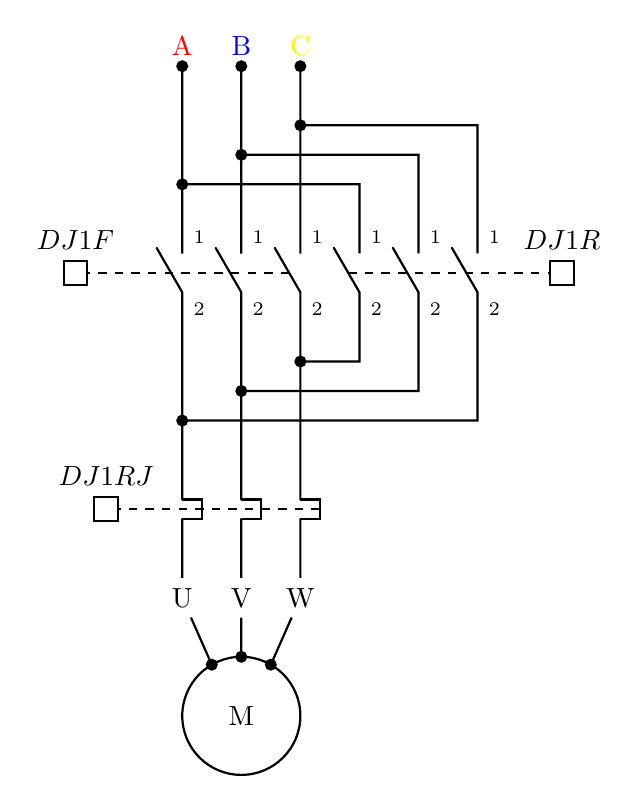
\begin{tikzpicture}[circuit ee IEC relay,thick,scale=1.5]

%d动力回路
\node (M) at (0.5,0) {M};%绝对坐标
\draw (0.5,1) node(V1) {V} %绝对坐标
	+(-0.5,0) node(U1) {U}
	+(0.5,0) node(W1) {W};

\draw (M) circle (0.5);

\draw (M) ++(120:0.5) node [contact,name=U]{};
\draw (M) ++(90:0.5) node [contact,name=V]{};
\draw (M) ++(60:0.5) node [contact,name=W]{};


\draw (V) -- (V1) -- ++(0,0.25)
to [thermic sensor] ++(0,1) -- ++(0,0.5)
node [contact,name=V2]{} -- ++(0,0.5)
to [make contact={term=1,term'=2}] ++(0,1) -- ++(0,0.5)
node [contact,name=V3]{} -- ++(0,0.75)
node [contact,name=V4]{};
\node[above,blue] at(V4) {B};

\draw (U) -- (U1) -- ++(0,0.25)
to [thermic sensor] ++(0,1) -- ++(0,0.25)
node [contact,name=U2]{} -- ++(0,0.75)
to [make contact={term=1,term'=2}] ++(0,1) -- ++(0,0.25)
node [contact,name=U3]{} -- ++(0,1)
node [contact,name=U4]{};
\node[above,red] at(U4) {A};

\draw (W) -- (W1) -- ++(0,0.25)
to [thermic sensor={name=FR}] ++(0,1) -- ++(0,0.75)
node [contact,name=W2]{} -- ++(0,0.25)
to [make contact={name=KM1,term=1,term'=2}] ++(0,1) -- ++(0,0.75)
node [contact,name=W3]{} -- ++(0,0.5)
node [contact,name=W4]{};
\node[above,yellow] at(W4) {C};

\draw (V2) -- ++(1.5,0) -- ++(0,0.5) to [make contact={term=1,term'=2}] ++(0,1) -- ++(0,0.5) -- (V3);

\draw (U2) -- ++(2.5,0) -- ++(0,0.75) to [make contact={term=1,term'=2}] ++(0,1) -- ++(0,0.75) -- (W3);

\draw (W2) -- ++(0.5,0) -- ++(0,0.25) to [make contact={name=KM2,term=1,term'=2}] ++(0,1) -- ++(0,0.25) -- (U3);


\draw[dashed](KM1.mid) -- ++(-1.7,0) node[left,draw,solid,minimum size=3mm,label={[above]:$DJ1F$}]{};

\draw[dashed](KM2.mid) -- ++(1.7,0) node[right,draw,solid,minimum size=3mm,label={[above]:$DJ1R$}]{};

\draw[dashed](FR.mid) -- ++(-1.7,0) node[left,draw,solid,minimum size=3mm,label={[above]:$DJ1RJ$}]{};




	\end{tikzpicture}
		\end{minipage}
}
\subfloat[控制回路]{
\label{fig:improved_subfig_b}
		\begin{minipage}{600pt}
\begin{tikzpicture}[circuit ee IEC relay,thick,x=8\tikzcircuitssizeunit,y=7\tikzcircuitssizeunit]
		
			\draw (0,0)node [contact,name=F1]{} -- ++(0,1) node [contact,name=G1]{}
				-- ++(0,1)node [contact,name=H1]{}
-- ++(0,1)node [contact,name=A1]{}
-- ++(0,1)node [contact,name=B1]{}
-- ++(0,1)node [contact,name=C1]{}
-- ++(0,1)node [contact,name=D1]{}
-- ++(0,1)node [contact,name=E1]{}
-- ++(0,1.2)node [contact,name=L]{};

	\draw (D1) -- ++(1,0)
		to [make contact={name=GK1,term=8-i}] ++(1,0)
		to [break contact={position switch={info=$LSR$}}] ++(1,0)
		node [contact,name=D2]{}
	to [make contact={info=$KA1J$}] ++(1,0) -- ++(1,0)
		to [break contact={info=$DJ1F$}] ++(1,0)
		to [relay coil={info=$DJ1R$,term=A2,term'=A1}] ++(1,0) 
		node [contact,name=D3]{};
	
				

		\draw (E1) node[contact]{}
		to [make contact={push button={info=$START$}}] ++(1,0)

		node [contact,name=E2]{}
		to [make contact={turn switch={info=$GK$},name=GK2}] ++(1,0)
		node [contact,name=E3]{}
		to [break contact={position switch={info=$LSF$}}] ++(1,0)
		to [break contact={info=OA1J}] ++(1,0)
		to [break contact={info=DJ1J}] ++(1,0)
		to [break contact={info=DJ1R}] ++(1,0)
		to [relay coil={info=DJ1F,term=A2,term'=A1}] ++(1,0)
		node [contact,name=E4]{};

\draw[dashed](GK1.mid) -- (GK2.mid);
\draw (E3) -- ++(0,-0.5) to [make contact={info={[right=0.3cm]:DJ1F}}] ++(1,0) -- (D2);
\draw (L) ++(1,0)node [contact,name=Di]{}--(E2);

		

		\draw (D2) -- ++(0,-1)
		to [break contact={info=DJ1F}] ++(1,0) -- ++(2,0)
		to [relay coil={info=DJ1J}] ++(1,0)
		node [contact,name=C3]{};
\draw (C3) -- (E4)
to [break contact={thermal switch={info=DJ1RJ}}] ++(0,1.2)node [contact,name=N]{};
\node[above,blue] at(N) {N};
\node[left,red] at(L) {A1};
\node[left,red] at(Di) {D-DJ1};

\draw (A1) -- ++(1,0)
to [break contact={info=OA1J}] ++(1,0)
to [make contact={info=DJ1J}] ++(1,0)
to [break contact={delayed deactivation={info=KT3}}] ++(1,0)
-- ++(2,0)
to [relay coil={slow operating={info=KT1}}]++(1,0)
node [contact,name=A2]{};

\draw (B1)
to [make contact={delayed deactivation={info=KT1}}] ++(1,0)
node [contact,name=B2]{}
to [relay coil={info=KA1J}] ++(1,0)
node [contact,name=B3]{}
-- ++(5,0)
node [contact,name=B4]{};

\draw (C1)
to [make contact={info=OA1J}] ++(1,0)
node [contact,name=C2]{}
to [relay coil={slow operating={info=KT3}}]++(1,0)
to (B3);

\draw (B2) -- (C2);

\draw (G1)
to [make contact={push button={info=$SB$,term''=现场急退}}] ++(2,0)
node [contact,name=G2]{};
\draw (H1)
to [make contact={info=$DCS$}] ++(2,0)
node [contact,name=H2]{}
-- ++(4,0)
to [relay coil={info=OA1J}] ++(1,0) -- (C3);
\draw (F1)
to [make contact={info=OA1J}] ++(1,0)
to [make contact={info=DJ1J}] ++(1,0) -- (H2);
%\draw (F2) -- (G2) -- (H2);
	\end{tikzpicture}
		\end{minipage}
}
\caption{空预器吹灰器电气回路图}
\label{fig:improved_subfig}
	\end{figure}
\end{center}
		\ifx \allfiles \undefined
\end{document}

\fi
